% A book summary template inspired by Jan Küster's Left Sidebar CV / https://github.com/jankapunkt/latexcv

\documentclass[11pt,a4paper]{article}	
\usepackage[utf8]{inputenc}	

% some tex-live fonts - choose your own

%\usepackage[defaultsans]{droidsans}
%\usepackage[default]{comfortaa}
%\usepackage{cmbright}
\usepackage[default]{raleway}
%\usepackage{fetamont}
%\usepackage[default]{gillius}
%\usepackage[light,math]{iwona}
%\usepackage[thin]{roboto} 

% set font default
\renewcommand*\familydefault{\sfdefault} 	
\usepackage[T1]{fontenc}

\usepackage{moresize}
\usepackage{fontawesome}

\usepackage{paracol}
\usepackage[margin=1.5cm]{geometry}

\usepackage{fancyhdr}
\pagestyle{empty}
\setlength{\parindent}{0mm}
\usepackage{graphicx}
	
\usepackage{tikz}				
\usetikzlibrary{shapes, backgrounds,mindmap, trees}

\usepackage{transparent}
\usepackage{color}

\definecolor{maincol}{RGB}{ 225, 0, 0 }
\definecolor{darkcol}{RGB}{ 70, 70, 70 }
\definecolor{lightcol}{RGB}{245,245,245}

\usepackage{enumitem}
\setitemize{label={\color{maincol}\faCheck}}

\usepackage[skip=\medskipamount]{parskip}
\usepackage{hyperref}
\hypersetup{
    backref=true,
    citecolor=magenta,
    colorlinks=true,
    linkcolor=blue,
    filecolor=magenta,
    urlcolor=cyan,
}
% A book summary template inspired by Jan Küster's Left Sidebar CV / https://github.com/jankapunkt/latexcv
% The following are the elements taken from said template, albeit from heading onwards was modified and made simpler or added as entirely new elements.



% use to vertically center content
% credits to: http://tex.stackexchange.com/questions/7219/how-to-vertically-center-two-images-next-to-each-other
\newcommand{\vcenteredinclude}[1]{\begingroup
\setbox0=\hbox{\includegraphics{#1}}%
\parbox{\wd0}{\box0}\endgroup}

% use to vertically center content
% credits to: http://tex.stackexchange.com/questions/7219/how-to-vertically-center-two-images-next-to-each-other
\newcommand*{\vcenteredhbox}[1]{\begingroup
\setbox0=\hbox{#1}\parbox{\wd0}{\box0}\endgroup}

% icon shortcut
\newcommand{\icon}[3] { 							
	\makebox(#2, #2){\textcolor{maincol}{\csname fa#1\endcsname}}
}	

% icon with text shortcut
\newcommand{\icontext}[4]{ 						
	\vcenteredhbox{\icon{#1}{#2}{#3}}  \hspace{2pt}  \parbox{0.9\textwidth}{\textcolor{#4}{#3}}
}

% icon with website url
\newcommand{\iconhref}[5]{ 						
    \vcenteredhbox{\icon{#1}{#2}{#5}}  \hspace{2pt} \href{#4}{\textcolor{#5}{#3}}
}

% icon with email link
\newcommand{\iconemail}[5]{ 						
    \vcenteredhbox{\icon{#1}{#2}{#5}}  \hspace{2pt} \href{mailto:#4}{\textcolor{#5}{#3}}
}

%---------------------------------------------------------
% MODIFIED from Kuester's CV
%---------------------------------------------------------
% Renders a a CV section headline with a nice underline in main color.
% param 1: section title
\newcommand{\heading}[1] {
	\vspace{15pt}
	{\bf\LARGE\color{darkcol}\uppercase{#1}}\\[-4pt]
	{\color{maincol}\rule{0.1\textwidth}{2pt} }\vspace{2pt}
}

%---------------------------------------------------------
% New 
%----------------------------------------------------------
\newcommand{\titlebox}[3]
{\fcolorbox{#1}{#2}{\begin{minipage}[c][4.5cm][c]{\linewidth}%
\begin{center}\large\color{white} #3 %
\end{center}\end{minipage}\\[14pt]
\vspace{-12pt}
}
}

\newcommand{\bigfont}[1]{%
{\bf\huge\uppercase{#1} } \\[4pt]%
\rule{0.1\textwidth}{1.25pt} \\[4pt]%
}

\newcommand{\titletext}[1]{%
#1 \\[4pt] %
\rule{0.1\textwidth}{1.25pt} \\[4pt]%
}

\renewenvironment{quote}
               {\list{\Large\color{black!50}\faQuoteLeft\phantom{ }}{\rightmargin\leftmargin}%
                \item\relax\Large\color{black!50}\ignorespaces}
               {\unskip\unskip\phantom{xx}\color{black!50}\faQuoteRight\normalsize\endlist}
           




\let\emph\textit % hopefully temporary: https://tex.stackexchange.com/a/350044/64425

%============================================================================%
\begin{document}
\columnratio{0.31}
\setlength{\columnsep}{2.2em}
\setlength{\columnseprule}{4pt}
\colseprulecolor{lightcol}
\begin{paracol}{2}

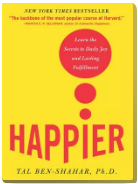
\includegraphics[width=\linewidth]{happier.png}

\heading{Overview}

\small

\icontext{Male}{12}{Greg McKeown}{black}\\[6pt]	
\icontext{Book}{12}{Essentialism: The Disciplined \\ Pursuit of Less}{black}\\[6pt]	
\icontext{MapMarker}{12}{NY}{black}\\[6pt]
\icontext{Calendar}{12}{2011}{black}\\[6pt]
\iconemail{Laptop}{12}{Book Website}{https://gregmckeown.com/book/}{black}\\[6pt]
\iconemail{Globe}{12}{Summary Source 1}{https://epigrammetry.hypotheses.org/595}{black}\\[6pt]
\iconemail{Globe}{12}{Summary Source 2}{https://epigrammetry.hypotheses.org/248}{black}\\[6pt]

\vspace{3em}

%\begin{figure}[h]
%    \centering
%    \includegraphics{essentialism-energy.png}
%    \caption{Graph illustrating how far you can go with the same amount of energy if invested deliberately in just one thing versus diffusion}
%    \label{fig:my_label}
%\end{figure}


\normalsize
\switchcolumn

\titlebox{white}{darkcol}{

\bigfont{Happier} 

\titletext{Tal Ben-Shahar}

Learn the Secrets to Daily Joy and Lasting Fulfillment
}
\vspace{1em}

%---------------------------------------------------------------------------------------


\heading{Summary}

The normal state of a closet is to get more and more cluttered if a conscious effort is not made to get rid of non-essentials. Consciously making this effort over and over again is what McKeown calls `disciplined'. 

\begin{quote}
    Essentialism is the disciplined pursuit of ‘less but better’.
\end{quote}

The clutter piles up again and every time it does, you need to act: You need to know where the next thrift store is and when it’s open. You need to have a plan in case somebody drops off their clutter in your closet.


\heading{Essentialist checklist}
\begin{itemize}
    \item Do less than you want to do / could do. 
    \item get enough sleep, drink enough water ('protect the asset')
    \item take time for 'serious play'
    \item If you don't know what’s important right now, what’s important right now is to find out what’s important right now. Only once you know this can you use your time effectively.
\end{itemize}

\heading{Actionable advice}
\begin{enumerate}
    \item 
    \textbf{Part two (“Explore”)} suggests you ‘escape’ and save time by being unavailable (ruthlessly avoid going to useless meetings, etc.); you see what really matters, make time for (serious) play, get enough sleep and select what you spend your time with using ‘extreme criteria’. 
    \item \textbf{Part III (“Eliminate”)} suggests you clarify decision making, dare to say no and learn how to do it gracefully without offending people, uncommit from non-essentials and gain freedom by setting boundaries for carefully ‘edited’ amount of meaningful activities.
    \item \textbf{Part IV (“Execute”)} praises using a “time buffer” between commitments, removing things which hurt your effectiveness most rather than starting some new quick fix technique on top of everything, progressing with small wins, using routine to get in the flow, focusing and being in the moment by asking (“What’s important now?”).
\end{enumerate}


\heading{Success spiral}

With clarity of purpose comes success. But with success come opportunities which distract you from your purpose and make you plateau. Now you have to subtract and say no politely. You only move forward if you put all your energy in the same direction. 


\heading{Essentialist mindset}
\begin{enumerate}
    \item There can only ever be one priority.
    \item Thus, trade-offs are real: you can either do this or that. By deciding on doing one thing, you discard the other. Make this an active choice.
    \item Remember the unimportance of practically everything: Say no and triage ruthlessly.
\end{enumerate}

You can't just fit it all in. Also, actions aren't all worth the same. Like in the Pareto principle (80/20), some actions have tremendously better effects than others which are practically useless in the pursuit of your goals. 

\heading {Detailed Notes}

The book is written in a self-help workbook style. You have got to do assignments (this is a stumbling block for readers and sometimes a marketing gimmick for authors -- but you should still spend time on them because, you know, you signed up for that). In this review an assignment and my take on it is shown as (Workout).

Details are described as a series of bullets.

\begin{enumerate}
    \item In Chapter 1, Ben urges you to find those instances in life where achieving a milestone did not bring you the \emph{emotional payoff} you expected.
    \item Upon being frustrated with experiencing ``emotional emptiness'' after Ben achieved a milestone of being an Israeli national squash champion at 16, he spent a lot of time pondering questions like:
        \begin{itemize}
            \item Do words like `bliss', `pleasure', `ecstasy', `contentment' mean the same thing as `happiness'?
            \item Can you be both happy and successful?
            \item Can you experience sadness at times and still enjoy overall happiness?
            \item How would you define happiness? What does it mean to you? (Workout) \\

                -- I think happiness (which derives from the Icelandic word `happ' meaning ``chance'' or ``luck'') is good health and poor memory ;-). Nah, just kidding. But among various definitions of happiness I like this the most: ``Happiness is not what happens to you, but what you make of it'' (here `it' refers to what happens to you).
        \end{itemize} 
    \item Ben espouses ``positive psychology'' throughout the book.
    \item ``Am I happy?'' is not a helpful question, but ``How could I be happier?'' may well be.
    \item Do daily rituals. 
    \item Keep a ``regularly maintained gratitude journal''. (Will I actually do it regularly? It's just writing five things that you felt or feel grateful about.) 

          -- I am a bit unclear about the value of doing this exercise. I believe in probability. Luck affects every one of us. As I sit here writing this, there are literally dozens of things and people (not the same, but variable, and sometimes even those whom I haven't met or seen) that I \emph{sincerely} think I am grateful for. Either I can say that I am grateful to them every now and then, or I can assume that \emph{most of} the people do their work enabling me to do my work. This is a ``graph'' where everyone depends on a few people directly and eventually on everyone else. So, what is the point of saying this \emph{explicitly} a hundred times regularly? This hinges on the ideas of faith and praying etc. Even when most of us do our assigned or accepted jobs, things can go seriously wrong for some of us and well, that's just beyond anyone's control in a universe which seems to be just indifferent. Gratitude is great, but not when you express it more-or-less habitually and conditionally. It is as if one should be grateful so that doing so will render one's life relatively painless.

             There could be some advantages of ``writing a journal'', but that does not have to repeatedly thank people and things that affect one's life.
    \item The Hamburger Model: Comprises of two axes -- benefit and detriment -- and four quadrants (archetypes):
        \begin{enumerate}
            \item Present detriment, future benefit -- Rat-race archetype
            \item Present detriment, future detriment -- Nihilism\footnote{One who has \emph{given up} happiness and has resigned to the belief that life has no meaning.} archetype
            \item Present benefit, future detriment -- Hedonism archetype
            \item Present benefit, future benefit -- Happiness archetype
        \end{enumerate}
    \item Write down when you were in each of the four quadrants (Workout).
    \item Meditate.
    \item Happiness is highest on the hierarchy of goals. Period. Wealth, fame, admiration, and all other goals are subordinate to happiness.
    \item Ask yourself the ``Infinitely regressive why'' -- why do you want to be happy? (Workout)
          
        -- Without formally defining happiness, this question is unanswerable. But if I go back to my definition of happiness -- it is \emph{not} what happens to you, but what you make of it -- then a good attempt can be made. In an uncertain world, if you feel like living and thriving every day (that is get up and do with enthusiasm something you truly like with all the frustrations it brings) and you are actually doing it for a long period of time, then you are doing it for the sake of it -- to make something of whatever happens to you. 

    \item Numerous studies show that happy individuals are successful across multiple life domains, including marriage, friendship, income, work performance, and health.
        
        -- Is the converse true? Perhaps not.

    \item Ben defines happiness as ``the overall experience of pleasure and meaning'': a person can endure emotional pain at times and still be happy overall.
        \begin{enumerate}
            \item Pleasure
                \begin{enumerate}
                    \item Antonio Damasio's patient, whose frontal lobe was damaged during a surgery retained his rational ability, but lost his emotional and feeling faculty, was a completely different being after the surgery. 
                    \item Emotion is the foundation of our motivation. 
                    \item However, merely being capable of emotion -- any emotion -- is not enough.
                    \item Even positive emotions are, though necessary, not sufficient for happiness.
                \end{enumerate}
            \item Meaning
                \begin{enumerate}
                    \item Would we want to circumvent the cause of our emotions? Perhaps yes. Most likely, we would want the cause of our emotions to be \emph{meaningful}. We want to know that our actions have an actual effect in the world, not just that we feel that they do.
                    \item While our capacity for emotions is similar to that of other animals, we are fundamentally different. We have the capacity of being conscious of our consciousness and our experiences. We are spiritual; the OED defines spirituality as ``the real sense of significance of something''.

                        -- Do I truly believe that? Can we explain the development of spirituality on the basis of biological evolution? How could I find evidence for the hypothesis that there were selection pressures for humans' spirituality? Is it that after at least a few of humans felt ``relatively safer'', these so-called ``higher faculty'' was developed? But then, how could we explain wars? If we fought wars so vehemently, how could we be conscious of our own consciousness?

                        -- Nonetheless, the above OED definition of spirituality sounds intriguing. It suggests that you may be spiritual in X if you have a \emph{real sense} of the significance of X. It also raises questions. Many a time, mathematicians don't have a real sense of the significance of something (because its significance may be realized a 100 years after they are gone) -- are they not leading a spiritual life then? Or am I taking it out of context? Ben has tried to explain it \href{https://wholebeinginstitute.com/leading-a-spiritual-existence/}{here}. He says that living spiritually means living in accordance with one's values (however, one's values can be worthless from another's point of view -- and that should be okay).
                \end{enumerate}
            \item An investment banker who finds pleasure and meaning in her work -- who is in it for the right reasons -- leads a more spiritual life than a monk who is in his field for the wrong reasons.

                -- Could it be that a certain gullibility is required to be spiritual? Chances are that if you are not knowing the ``dark side'' of something then you believe that there is no dark side to it. Consider that you are a chemist whose only interest is chemistry in general and the chemistry of detonators in particular. You keep to yourself and sell your services without choosing to know for what purpose they are used; you tend to just assume that they are for the good and not for the evil. But you do not investigate if it is indeed so because that is ``none of your business''. It turns out that some terrorists use your service indirectly. Were you still leading a spiritual life then? 

                -- Lives of spies, investors, soldiers, software programmers, and, I suspect, many others have this contrast all the time. Should you just rely on your expertise and satisfy your customers by being professional in your dealings or must you ensure that your expertise are also used by others (in a chain) for something ``good''?
        \end{enumerate}
    \item Idealism and Realism

        An overarching ``purpose'' can, like a grand unification principle, unify individual activities.

    \item Potential and Happiness

        We have an inborn desire to know (to quote Aristotle: ``All men, by nature, desire to know.'').

        ``The happiness that is genuinely satisfying, is accompanied by the fullest exercise of our faculties and the fullest realization of the world we live in.'' -- Bertrand Russell

        We can find satisfaction if we feel from within that we are doing things that challenge us and utilize us fully and well.

        -- I think I agree with that. We want to know. We are curious. I am not so sure if this is natural or inborn -- Could it be that, like John Locke has said in his essay on human understanding, we attain this faculty by observation? I do believe that most of us have the capacity to know, however. Perhaps other animals do not have such a capacity. 
        -- According to Viktor Frankl, fulfillment of potential is meaningful.
        \begin{enumerate}
            \item (Workout) What pursuits would challenge you and fulfill your potential?

                -- This is a trick question. A monomaniacal pursuit of any one thing has been my problem. On the one hand, I believe that I am a multipotentialite (a person who has multiple talents but none of them are perhaps very good; a glorified jack of many trades and master of none) and I like that ``range'' of possibilities (that I can be any one of those), but, on the other hand, it feels too fleeting, too incomplete. I tend to spend serious time in getting better at one or two of those things (at the cost of others), but the progress has been elusive. Progress has at least been not as `quick' as I'd like. That is understandable; world-class expertise needs a lot of things to come together. One of those things is the focused time during which you may find yourself in the `flow' (as defined by Csikszentmihalyi). It is clear that I have not been any `flow' in my life. Or is it that I just don't want to take up the crucial sacrifices that come with the development of expertise? I don't know.

                -- But that should not deter me from picking the things that I believe may fulfill my potential:

                -- Programming, problem-solving, learning science

                -- Teaching

                -- Writing

                -- Playing (chess, cricket, and badminton)

                -- But I am not sure if any of these are ``employable'' or ``recognizable'' traits. Fortunately, I don't yet need to be employable, but it does feel like these are my not-so-serious hobbies.  
        \end{enumerate}
    \item Success and Happiness

    \item The Need for Meaning and Pleasure

        -- We have got to reference MSFM somewhere.

        -- Ben's ``theory of happiness'' derives from both Freud's pleasure principle and Frankl's ``will to meaning''.
    \item Mapping Your Life (Workout)
    \item Integrity Mirror
    \item The Ultimate Currency
        \begin{enumerate}
            \item Marva Collins's story as a Chicago school founder. ``Teaching Tiffany (an autistic child that experts declared as an unlovable and unteachable child) and helping her succeed in life'' was worth all the gold in Fort Knox for Marva.
            \item ``Teaching'' gave her life meaning that no other profession could give.
            \item (Workout) What for you is worth all the gold in Fort Knox?

                -- This does come as a great question that is ``in your face''. I can't escape it. Really, for me, what is worth all the gold in Fort Knox? Is it my meager achievements, my family, or my knowledge (which is limited)?

                -- Of course, the apparent rhetoric of something (you value) on the one hand and all that gold on the other makes the question dramatic. It really means to ask, ``What do you value the most?''

                -- Often such a thing is your achievement: For Marva, it was Tiffany's (and perhaps many others') resounding success that Marva, against all odds, helped her achieve (Tiffany's success became Marva's treasure). If you don't value any of your own achievements highly (or that highly) then what will you weigh? If you have led more-or-less normal (within $\pm 2\sigma$) life, it is likely that you draw a blank as you look for something invaluable.

                -- I also think that there is no requirement that what you value the most be outstanding, only that you honestly believe that is worth its weight in gold.

                -- Maybe it's the freedom (of thoughts), unconventionality. I tend to think independently, sometimes to my own predicament and that of others around me. But I seem to value this trait, perhaps partly because I don't see it in the society. It's unclear if I value it because it makes me stand out or because I truly value it. Nonetheless, it's my ability to think independently, sometimes to the extent of being judged heretical, that I would hesitate to give up for any amount of pure gold. 

                -- I also think that I am not a ``great man'' (in a somewhat abstract sense) -- a revered figure, a hero of sorts -- who makes a difference to others' lives. Such a person may start out with a mild goal of becoming great at something. I certainly do not want to do it against my objective wishes, just because it is somehow branded ``good''. I like to help people very much, but I am not always sure if someone needs help. Maybe something like what Marva did (founding a school, a nonprofit or even for-profit business, writing an app or contributing to the open source software development, teaching) where you do things for your own sake and, as a side effect, others get benefited is the way to go about it. But doing something ``for society'' is not what comes naturally to me. I can only help others by helping myself, not the other way round.
        \end{enumerate}
    \item Happiness as the Ultimate Currency

          -- The example of ``A conversation with a friend or a million dollars?'' appears far-fetched.

      \item Wealth and Happiness

          David Myers found very little correlation between material wealth and happiness, except in cases of extreme poverty where people's basic needs weren't being met.

          Some people feel more depressed once they have attained material property than they did while striving for it.

          In spite of this, why does being rich so often takes precedence over finding meaning? ... It's related to our evolutionary past, maybe? Hoarding became a part of our constitution. This evolved into seeking material well-being: We no longer accumulate to live; we live to accumulate.

          ``Society tells us that the only thing that matters is matter, the only things that count are the things that can be counted.'' -- Laurence G. Boldt in Zen and the Art of Making a Living.

          (Workout) Does a concern over wealth and prestige detract you from overall experience of happiness? In what ways?

          -- I steach (study+teach) with my kids in our fun-loving, science-based home school (Tell me, does that scare you or turn you off?). In order to steach, about a year ago I left a peaceful and very well-paying job that was fun about half the time. Do I regret it? I don't think so. I mean, I quit it after some financial planning with my very capable wife and I am living off my investments and sometimes the thought of a salaried job does linger in my mind, but I am able to quickly get over it. My current job pays me no salary, but it is fun almost all the time. Thus, I think that a stable life is, although characterized by a ``negative cash-flow'' in the present, well worth living. There are no regrets about the lost material superiority. Why do I not forget that I had such a well-paying job then? I have to be honest and tell you the truth that I do sometimes remember it, but it is equally true that I don't regret it. In the last one year, I have learned so much science and so much about education and child psychology!
          
      \item Emotional Bankruptcy

          While we are making huge strides in science and technology -- in our material welfare -- we are rapidly falling farther and farther behind emotionally.

          Emotional Bankruptcy -- The ``overwhelming hopelessness'' -- the nihilism that [Daniel] Goleman describes -- results from our sense that we are unable to overcome this impoverished emotional state, on either the individual or the global level.

      \item (Workout) Sentence Completion
          \begin{enumerate}
              \item A technique developed by psychotherapist Nathaniel Branden -- Simply generating a number of endings to an incomplete sentence -- often helps people come up with insights that bring about meaningful change in their lives. You can do this in writing or on a sound recorder. Examples: ``If I bring 5 percent more awareness to my life \dots'', ``The things that make me happy are \dots''
          \end{enumerate}
      \item Setting Goals
            \begin{quote}
                Happiness grows less from the passive experience of desirable circumstances than from involvement in valued activities and progress toward one's goals.
            \end{quote}
        \item Goals and Success
          \begin{enumerate}
              \item (Although I didn't believe it before and attainment of goals early in life made me emotionally bankrupt), today I believe that goals are indispensable to a happy life -- to be happy we need to identify and pursue goals that are both pleasurable and meaningful.
              \item Setting a goal is about making a commitment in words, and words have the power to create a better future.
              \item (Workout) Think of an experience or two where you committed to something. What were the consequences of your commitment? What are you committed to now?

                  -- Serious commitments have all been in younger or student life. The consequences have been good in the short term. 

                  -- Right now I am committed to teaching my kids and learning mathematics and science myself. The main commitment is to do what homeschooling requires me to do. I am committing to learning geometry, calculus, physics-2, Sanskrit, and English grammar.

              \item The Role of Goals
                  
                  The proper role of goals is to liberate us, so that we can enjoy the here and now. 

               \item (Workout) What goals have provided you with the most happiness in the past, in terms of facilitating as well as meaningful journey? What goals do you believe will do the same for you in the future?

               \item Self-Concordant (Matching) Goals

                   Those that we pursue out of deep personal conviction and/or a strong interest. They are ``integrated with the self''.

                   While there are clearly many benefits to \underline{identifying} and \underline{pursuing} self-concordant goals, it is anything but easy.

                   ``Selecting self-concordant goals is a difficult skill, requiring both accurate (dependable?) self-perpetual abilities and the ability to resist social pressures that may sometimes push one in inappropriate directions.'' -- Sheldon and Linda Houser-Marko. 

               \item Want-to Vs. Have-to

                   `Want-to' goals are self-concordant. `Have-to' goals are more like chores, although one may still find meaning in them. How happy I am depends to a large extent on the ratio between want-tos and have-tos in my life. 

                   -- In this regard, I keep reminding myself of this quote:

                   -- ``There are two ways to wash the dishes. The first way is to wash the dishes in order to have clean dishes and the second is to wash the dishes to wash the dishes'' -- Thich Nhat Hanh

                   -- Overall, this makes sense, but there's nothing original in this discussion. There's also these concentric-looking circles that are labeled `Can do', `Want to do', `Really want to do', and `Really, really want to do' that are supposed to help you decide. But it still does not make the point clear. There is a beautiful zen story that elucidates the point effectively, maybe Ben should've used that story here.

		   -- Anyway, I decided to write down my goals in a way that helps me schedule events on my calendar. It rarely happens in one go; one needs to have several drafts before finally committing to something.
          \end{enumerate}

\end{enumerate}


\end{paracol}
\end{document}
